\section{Auswertung}
\label{sec:Auswertung}

Zunächst wird die in der Durchführung (\ref{sec:d0}) beschriebene Justierung durchgeführt.
Nach Bestimmung der Resonanzfrequenz des fest justieren Stromkreises sowie der Jusitierung des regelbaren Stormkreises ergibt sich eine Resonanzfrequenz von
\begin{align*}
\nu_{\text{resonanz}} = \SI{30.49}{\kilo\hertz}.
\end{align*}

\subsection{Bestimmung der Schwebungsfrequenzen}
Das Verhältnis der Resonanzfrequenzen $\omega_r$ und der Schwebungsfrequenzen $\omega_s$ wird, wie in der Durchführung (\ref{sec:d1}) beschrieben sowie in Abbildung \ref{fig:4} skizziert, bestimmt.
Dabei werden dem Versuchsaufbau die Werte
\begin{align*}
  L &= \SI{32.351}{\milli\henry} \\
  C &= \SI{0.8015}{\nano\farad} \\
  C_{\text{sp}} &= \SI{0.037}{\nano\farad} \\
  \increment C_k &= \SI{\pm 0.5}{\percent}
\end{align*}
entnommen.
Tabelle \ref{tab:1} gibt die Messdaten sowie Theoriewerte an.

%\OverfullCenter{
\begin{table}
  \centering
  \caption{Messdaten für die Messung der Schwebungsfrequenzen}
  \label{tab:1}
  \sisetup{table-format=3.4}
  \begin{tabular}{c c c c c c c c c c c c}
    \toprule
    {$N$} & {$\increment N $} & {$ C_k [\si{\nano\farad}] $} & {$\increment C_k [\si{\nano\farad}] $} & {$ \omega_r [\si{\kilo\second\tothe{-1}}] $} & {$\increment \omega_r [\si{\kilo\second\tothe{-1}}] $} & {$ \omega_s [\si{\kilo\per\second}] $} & {$\increment \omega_s [\si{\kilo\per\second}] $} & {$\frac{\omega_r}{\omega_s}_{\text{}}$} & {$\increment \frac{\omega_r}{\omega_s}_{\text{}}$} & {f [\%]} \\
    \midrule
    \input{build/wr_ws_verhaeltnis.tex}
    \bottomrule
  \end{tabular}
\end{table}
%}


Hierbei beschreibt $N$ die Anzahl der Maxima der Resonanzfrequenz pro halber Persiode der Schwebungsfrequenz, $C_K$ beschreibt die jeweils betrachtete Justierung des Koppelkondensators $C_k$.
Die Werte für $\omega_r$ und $\omega_s$ berechnen sich nach \eqref{eqn:omega_s} und \eqref{eqn:omega_r}, $\frac{\omega_r}{\omega_s}$ gibt das Verhältnis der beiden theoretischen Größen an.
Zuletzt wird die relative Abweichung
\begin{equation}
f = \frac{\lvert N - x \rvert }{x}
\label{eqn:rel_err}
\end{equation}
mit $x = \frac{\omega_r}{\omega_s}$ der experimentell abgelesenen Werte zu den Theoriewerten angegeben.\\

Die hier berechneten Fehler sowie alle folgenden fehlerbehafteten Messgrößen berechnen sich nach dem Gaußschen Fehlerfortpflanzungsgesetz
\begin{equation}
\increment{f} = \sqrt{\Bigl(\frac{\partial f}{\partial x_1}\increment{x_1}\Bigr)^2 + \Bigl(\frac{\partial f}{\partial x_2}\increment{x_2}\Bigr)^2 + \dotsc + \Bigl(\frac{\partial f}{\partial x_n}\increment{x_n}\Bigr)^2}
\end{equation}
für eine Funktion $f(x_1,x_2, \dotsc ,x_n)$, bei der die Größen $x_1, x_2, \dotsc , x_n$ voneinander unabhängig sind.
Für den Fehler von $\omega_r$ von $\omega_s$ ergibt sich die Fehlerformel
\begin{equation}
\increment{\omega_{r/s} = \frac{1}{ C_k^2 L \sqrt{ \frac{\frac{1}{C} + \frac{2}{C_k }}{L} } }   \increment{C_k}}.
%  \increment{\omega_r} = \sqrt{ \Biggl( \frac{1}{2} \biggl( \frac{-C}{2 \sqrt{LC}^3 } - \frac{\frac{1}{C} + \frac{2}{C_k} }{2 L^2 \sqrt{ \frac{\frac{1}{C} + \frac{2}{C_k }}{L} } } \biggr)   \increment{L} \Biggr)^2 + \Biggl( \frac{1}{2} \biggl( \frac{-L}{2 \sqrt{LC}^3 } - \frac{1}{2 C^2 L \sqrt{ \frac{\frac{1}{C} + \frac{2}{C_k }}{L} } } \biggr)   \increment{C} \Biggr)^2  + \Biggl(\frac{-1}{ C_k^2 L \sqrt{ \frac{\frac{1}{C} + \frac{2}{C_k }}{L} } } \biggr)   \increment{C_k} \Biggr)^2   }
\end{equation}
Bei dem direkten Vergleich der Theoriewerte mit den abgelesenen Werten fällt eine systematische Abweichung auf, so dass $N$, abgesehen von den beiden Kondensatoren mit den größen Kapazitäten, eine Abweichung nach unten besitzt.
Um diesen Fehler zu beheben, wird nun bei der Berechnung der Theoriewerte ebenfalls die reale Kapazität $C_{\text{sp}}$ der Spule berücksichtigt.
Im Gegensatz zu \eqref{eqn:omega1} und \eqref{eqn:omega1} ergeben sich nun für die korrigierte Bestimmung
\begin{equation}
  \omega_{1'} = \frac{1}{\sqrt{L(C+C_{\text{sp}})}}
  \label{eqn:omega1_neu}
\end{equation}
sowie
\begin{equation}
  \omega_{2'} = \sqrt{\frac{ \frac{1}{C+C_{\text{sp}}} + \frac{2}{C_k} }{ L }}.
  \label{eqn:omega2_neu}
\end{equation}
Hiermit ergeben sich die in Tabelle \ref{tab:2} angegebenen Werte.
\begin{table}
  \centering
  \caption{Messdaten für die Messung der Schwebungsfrequenzen unter Berücksichtigung von $C_{\text{sp}}$}
  \label{tab:2}
  \sisetup{table-format=3.4}
  \begin{tabular}{c c c c c c c c c c c c}
    \toprule
    {$N'$} & {$\increment N' $} & {$ C_k' [\si{\nano\farad}] $} & {$\increment C_k' [\si{\nano\farad}] $} & {$ \omega_r' [\si{\kilo\second\tothe{-1}}] $} & {$\increment \omega_r' [\si{\kilo\second\tothe{-1}}] $} & {$ \omega_s' [\si{\kilo\per\second}] $} & {$\increment \omega_s' [\si{\kilo\per\second}] $} & {$\frac{\omega_r'}{\omega_s'}_{\text{}}$} & {$\increment \frac{\omega_r'}{\omega_s'}_{\text{}}$} & {f' [\%]} \\
    \midrule
    \input{build/wr_ws_verhaeltnis_neu.tex}
    \bottomrule
  \end{tabular}
\end{table}

\subsection{Bestimmung der Fundamentalfrequenzen}

Die Fundamentalfrequenzen werden, wie in der Durchführung (\ref{sec:d2}) beschrieben mithilfe von Lissajous-Figuren bestimmt.
In Tabelle \ref{tab:3} werden die gemessenen Fundamentalfrequenzen $\nu_{1,\text{gem}}$ und $\nu_{2,\text{gem}}$ sowie die mit Hilfe von \eqref{eqn:omega1_neu} und \eqref{eqn:omega2_neu} bestimmten Werte $\nu_{1,\text{ber}}$ und $\nu_{2,\text{ber}}$ angegeben.
Zusätzlich wird die relative Abweichung der gemessenen zu den berechneten Frequenzwerten nach \eqref{eqn:rel_err} berechnet und angegeben.
\begin{table}[H]
  \centering
  \caption{Gemessene und berechnete Frequenzen}
  \label{tab:3}
  \sisetup{table-format=2.2}
  \begin{tabular}{c c c c c c c}
    \toprule
    {$\nu_{1,\text{gem}} [\si{\kilo\hertz}]$} & {$\nu_{1,\text{ber}} [\si{\kilo\hertz}]$} & {$f [\%]$} & {$\nu_{2,\text{gem}} [\si{\kilo\hertz}]$} & {$\nu_{2,\text{ber}} [\si{\kilo\hertz}]$} & {$\increment f_{2,\text{ber}} [\si{\kilo\hertz}]$} & {$f [\%]$} \\
    \midrule
    \input{build/vergleichdirekt.tex}
    \bottomrule
  \end{tabular}
\end{table}
Der Fehler von $\nu_{2,\text{ber}}$ berechnet sich zu
\begin{equation}
\increment{\nu_{2,\text{ber}}} = \frac{1}{2 \pi\, C_k^2 L \sqrt{ \frac{\frac{1}{C+C_s} + \frac{2}{C_k}}{L} } } \increment{C_k}.
\end{equation}

\subsection{Bestimmung eines Frequenzspektrums}
Das Frequenzspektrum wird, wie in der Durchführung (\ref{sec:d3}) beschrieben, aufgenommen.
Der Koppelkondensator wird bei der durchgeführten Messung auf $C_k = \SI{1.01}{\nano\farad}$ eingestellt.
Der Frequenzgenerator erzeugt dabei eine Sinusspannung der Amplitude $U_0 = \SI{30}{\volt}$.
Innerhalb von einer Sekunde durchläuft der Frequenzgenerator den Bereich von $\nu_{\text{start}}$ bis $\nu_{\text{end}}$ mit
\begin{align*}
  \nu_{\text{start}} &= \SI{14.75}{\hertz} \\
  \nu_{\text{end}} &= \SI{84.39}{\kilo\hertz}.
\end{align*}
Die Peaks treten für
\begin{align*}
  \tau_1 &= \SI{360}{\milli\second} \\
  \tau_2 &= \SI{552}{\milli\second}.
\end{align*}
auf, wobei $\tau_1$ die Zeit vom Beginn des Frequenzdurchlaufes zum ersten Peak ist sowie $\tau_2$ die Zeit bis zum zweiten Peak.
Hieraus lassen sich die Frequenzen der Peaks bestimmen zu
\begin{align*}
  \nu_1 &= \SI{30395}{\hertz} \\
  \nu_2 &= \SI{46590}{\hertz}.
\end{align*}
Berechnet man zusätzlich die zu diesen Frequenzen erreichten Stromwerte, so erhalten wir nach \eqref{eqn:idoof}
\begin{align*}
  I_{2,1} &= \SI{0.0155}{\ampere} \\
  I_{2,2} &= \SI{0.0103}{\ampere}.
\end{align*}
%
%
%
%
%\begin{figure}
%  \centering
%  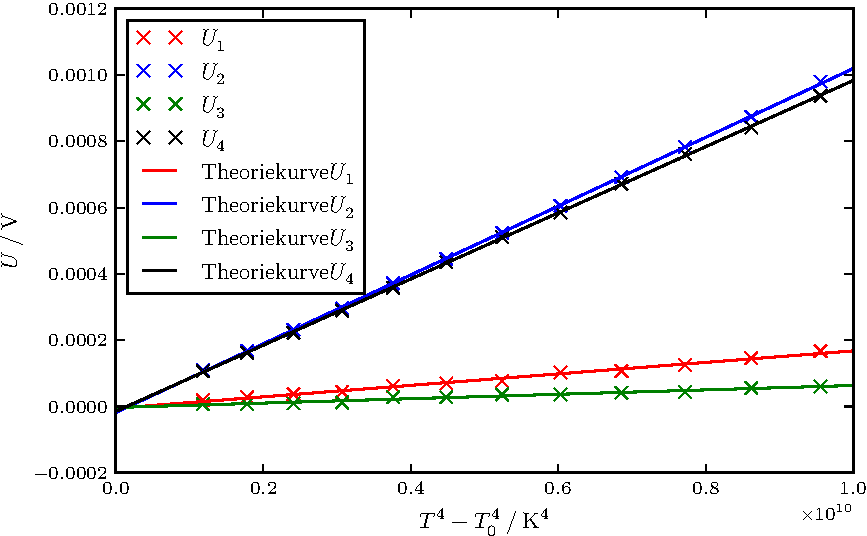
\includegraphics{plot.pdf}
%  \caption{Plot.}
%  \label{fig:plot}
%\end{figure}
%
%\begin{table}
%  \centering
%  \caption{Beispieltabelle}
%  \label{tab:tabelle_beispiel}
%  \sisetup{table-format=1.2}
%  \begin{tabular}{c c}
%    \toprule
%    {$a [\si{\second}]$} & {$b [\si{\kelvin}]$}\\
%    \midrule
%    1.0000  & 11.00 \\
2.0000  & 12.00 \\
3.0000  & 13.00 \\
4.0000  & 14.00 \\
5.0000  & 15.00 \\
6.0000  & 16.00 \\
7.0000  & 17.00 \\
8.0000  & 18.00 \\
9.0000  & 19.00 \\
10.0000 & 20.00 \\

%    \bottomrule
%  \end{tabular}
%\end{table}
%
%Es ergibt sich
%\begin{align}
%  a &= (0 \pm 0) ~ \si{\joule\per\kelvin\per\gram}
 \\
%\end{align}
%
